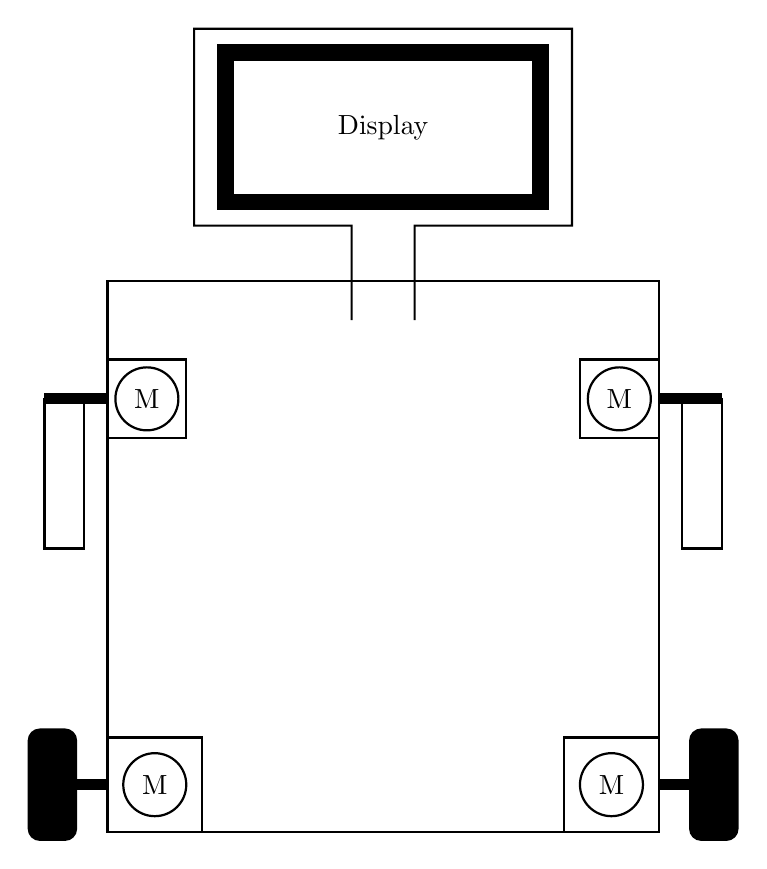
\begin{tikzpicture}[thick]
	
	%\draw (0,0) rectangle (10,10);
%	
%	\draw[fill=blue!55] (-0.9,1.4) circle (0.5);
%	\draw[fill=blue!55] (-0.8,1.3) circle (0.5);
%	
%	%xscale=-1
%		\draw[fill=lightgray!55] (0,0) rectangle (3,3);
%		\draw[fill=lightgray!55] (0,0) -- ++ (-1.5,1.5) -- ++ (0,3) -- ++ (3,0) -- ++ (1.5,-1.5) -- ++ (-3,0) -- ++ (0,-3);
%		\draw (0,3) -- ++ (-1.5,1.5);
%		
%		\draw[fill=blue!55] (0.6,0) circle (0.5);
%		\draw[fill=blue!55] (0.7,-0.1) circle (0.5);
%		\draw[fill=blue!55] (0.7,-0.1) circle (0.2);
%		\draw[fill=blue!55] (0.75,-0.15) circle (0.2);
%		
%		\draw[fill=blue!55] (2.4,0) circle (0.5);
%		\draw[fill=blue!55] (2.5,-0.1) circle (0.5);
%		\draw[fill=blue!55] (2.5,-0.1) circle (0.2);
%		\draw[fill=blue!55] (2.55,-0.15) circle (0.2);
		\begin{scope}[shift={(0,0)}] 
		\draw[rounded corners,fill=black]
		(-1,0.6+0.7) rectangle (-0.4,0.6-0.7);
		\draw[line width=4] (0,0.6) -- ++ (-0.4,0);
		%Reifen Rechts
		\draw[rounded corners,fill=black]
		(7+1,0.6+0.7) rectangle (7+0.4,0.6-0.7);
		\draw[line width=4] (7,0.6) -- ++ (+0.4,0);
		
		
		\draw[] (0,0) rectangle (7,7);
		%Motoren
		\draw[] (0,0) rectangle (1.2,1.2);
		\draw[] (0.6,0.6) circle (0.4) node[align=center] {M};
		
		\draw[] (5.8,0) rectangle (7,1.2);
		\draw[] (6.4,0.6) circle (0.4) node[align=center] {M};
		
		
		
		
		\end{scope}
		
		\begin{scope}[shift={(0,+5)}] 
		%Arne
		\draw[] (0,0) rectangle (1,1);
		\draw[] (0.5,0.5) circle (0.4) node[align=center] {M};
		
		\draw[] (6,0) rectangle (7,1);
		\draw[] (6.5,0.5) circle (0.4) node[align=center] {M};
				
				
		\draw[]
		(-0.8,0.5) rectangle (-0.3,0.6-2);
		\draw[line width=4] (0,0.5) -- ++ (-0.81,0);
		%Reifen Rechts
		\draw[]
		(7+0.8,0.5) rectangle (7+0.3,0.6-2);
		\draw[line width=4] (7,0.5) -- ++ (+0.81,0);
		\end{scope}
		
		
		\begin{scope}[shift={(0,0)}] 
		%	Kopf	♫
		\draw[] (3.5-0.4,6.5) -- ++ (0,1.2) -- ++ (-2,0) -- ++ (0,2.5) -- ++ (4+0.8,0) -- ++ (0,-2.5) -- ++ (-2,0)-- (3.5+0.4,6.5);
		
		%Display
		\draw[line width=6pt]
		(1.5,8) rectangle (5.5,9.9)
		node[midway, align=center] {Display};
	
	
		\end{scope}
		

		
		
		
		
		
		
		

\end{tikzpicture}